\documentclass[t,24pt]{beamer}

\usepackage[english]{isodate}
\usepackage{KUstyle}
\usepackage{multicol}
\usepackage{amsthm}
\usepackage{amsfonts}
\usepackage{amsmath}
\usepackage{amssymb}
\usepackage[normalem]{ulem}
\usepackage{tikz}
\usepackage{xcolor}

\renewcommand{\arraystretch}{1.25}
\toplinje{Parallel LL Parsing}

\begin{document}

{
\setbeamertemplate{background}{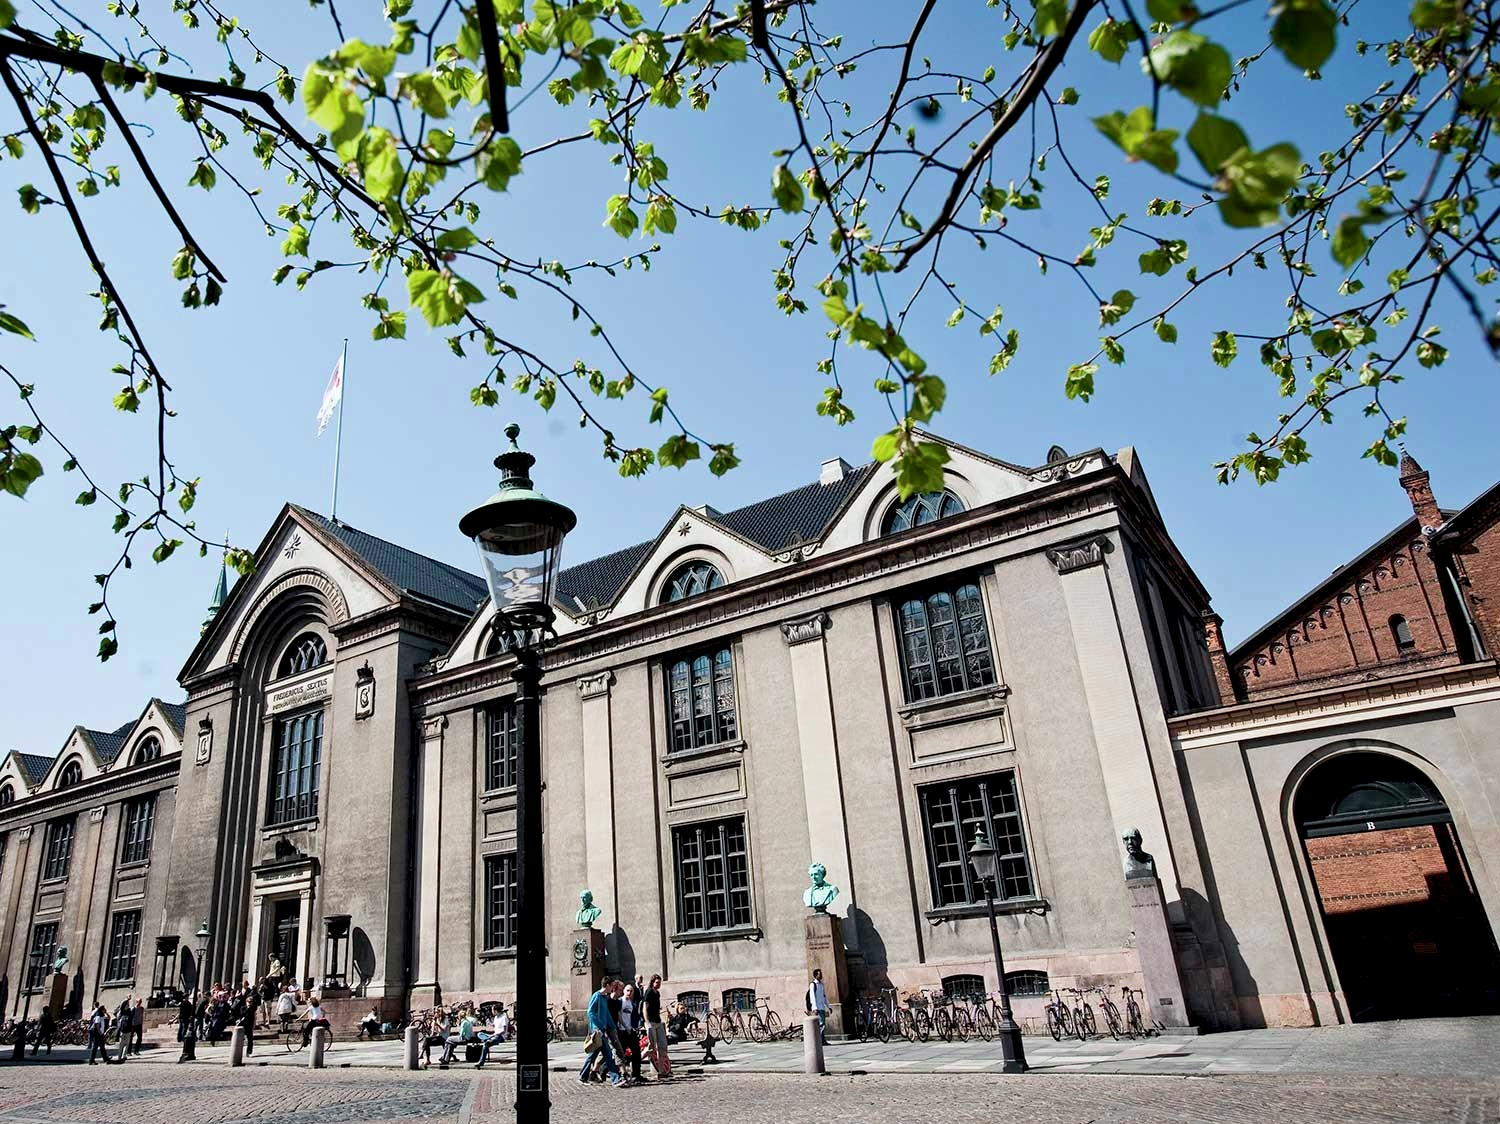
\includegraphics[width=\paperwidth,height=\paperheight]{images/frontpage.jpg}}
\begin{frame}
    \begin{textblock*}{\textwidth}(0.57\textwidth,0.1\textheight)
        \begin{beamercolorbox}[wd=6.4cm,ht=7.7cm,sep=0.5cm]{hvidbox}
            \fontsize{4}{10}\fontfamily{ptm}\selectfont \textls[200]{KØBENHAVNS UNIVERSITET}
            \noindent\textcolor{KUrod}{\rule{5.4cm}{0.4pt}}
        \end{beamercolorbox}
    \end{textblock*}
    \begin{textblock*}{\textwidth}(0.57\textwidth,0.1\textheight)
        \begin{beamercolorbox}[wd=6.4cm,sep=0.5cm]{hvidbox}
            \Huge \textcolor{KUrod}{Parallel Parsing}
            \vspace{0.5cm}
            \par
            \Large The Implementation of a Parallel LL Parser Generator
            \vspace{0.5cm}
            \par
            \normalsize William Henrich Due
            \vspace{0.1cm}
            \par
            30rd June 2023
        \end{beamercolorbox}
    \end{textblock*}
    \begin{textblock}{1}(14.2,11.44)
        
\includegraphics[width=1cm]{KU/KU-logo.png}
    \end{textblock}
\end{frame}
}

\begin{frame}[hvid]
    \frametitle{What did I do?}
\end{frame}

\begin{frame}[hvid,noframenumbering]
    \frametitle{LL parsing}
    Here is a LL(1) grammar.
    \begin{align*}
        1)\:\: T \to R \qquad 2)\:\: T \to aTc \qquad 3)\:\: R \to \varepsilon \qquad 4)\:\: R \to bR
    \end{align*}
    \begin{align*}
        \onslide<2->{(abc, T, ())} & \onslide<3->{\vdash (abc, aTc, 2)} \onslide<4->{\vdash (bc, Tc, 2)} \onslide<5->{\vdash (bc, Rc, (2, 1))} \\
                                   & \onslide<6->{\vdash (bc, bRc, (2, 1, 4))} \onslide<7->{\vdash (c, Rc, (2, 1, 4))}                         \\
                                   & \onslide<8->{\vdash (c, c, (2, 1, 4, 3))} \onslide<9->{\vdash (\varepsilon, \varepsilon, (2, 1, 4, 3))}
    \end{align*}
    \onslide<9->{Accepted! the string ``$abc$'' can be parsed.}
\end{frame}

\begin{frame}[hvid]
    \frametitle{LLP Parsing}
    Augment the grammar, this grammar is LL(1) and LLP(1, 1).
    \begin{align*}
        0)\:\: T' \to \:\: \vdash T \dashv
    \end{align*}
    Now we parse the string ``$\vdash abc \dashv$'' instead.
    \begin{center}
        \begin{tabular}{c|c|c|c|c}
            (\varepsilon ,\vdash) & $(\vdash, a)$ & $(a, b)$        & $(b, c)$             & $(c, \dashv)$               \\ \hline
            $(T',T\dashv,0)$      & $(T, Tc, 2)$  & $(T, R, (1,4))$ & $(Rc,\varepsilon,3)$ & $(\dashv, \varepsilon, ())$
        \end{tabular}
    \end{center}
    \onslide<2->{
        \begin{enumerate}
            \item Initial pushdown store.
            \item Final pushdown store.
            \item Left parse.
        \end{enumerate}
    }
\end{frame}
\begin{frame}[hvid]
    \frametitle{LLP Parsing using Parallel Reduce}
    Use the \uline{associative} $\mathbf{glue}$ operation.
    \vfill
    \begin{center}
        \begin{tikzpicture}[
                level distance=1cm,
                level 1/.style={sibling distance=3cm},
                level 2/.style={sibling distance=4cm},
                level 3/.style={sibling distance=2cm}]
            \node {$({\only<5>{\color{orange}} T'}, {\only<5>{\color{blue}} \varepsilon}, {\only<6>{\color{red}} (0, 2, 1, 4, 3)})$}
            child {node {$({\only<5>{\color{orange}} \only<4>{\color{orange}} T'}, {\only<4>{\color{green}} \only<5>{\color{red}} \dashv}, (0, 2, 1, 4, 3))$}
                    child {node {$({\only<4>{\color{orange}} \only<2>{\color{orange}} T'}, {\only<4>{\color{red}} \only<2>{\color{blue}} Tc}{\only<4>{\color{green}} \only<2>{\color{green}}\dashv}, (0, 2))$}
                            child {node {$({\only<2>{\color{orange}} T'}, {\only<2>{\color{red}} T} {\only<2>{\color{green}} \dashv},0)$}}
                            child {node {$({\only<2>{\color{red}} T}, {\only<2>{\color{blue}} Tc}, 2)$}}
                        }
                    child {node {$({\only<4>{\color{red}} \only<3>{\color{blue}} T} {\only<4>{\color{red}} \only<3>{\color{green}} c}, {\only<4>{\color{blue}} \only<3>{\color{orange}} \varepsilon}, (1,4,3 ))$}
                            child {node {$({\only<3>{\color{blue}} T}, {\only<3>{\color{red}} R}, (1,4))$}}
                            child {node {$({\only<3>{\color{red}} R}{\only<3>{\color{green}} c}, {\only<3>{\color{orange}} \varepsilon},3)$}}
                        }}
            child {node {$({\only<5>{\color{red}} \dashv}, {\only<5>{\color{blue}} \varepsilon}, ())$}};
        \end{tikzpicture}
    \end{center}
    \vfill
\end{frame}
\begin{frame}[hvid]
    \frametitle{LLP Parsing using Bracket Matching}
    \begin{center}
        \begin{tabular}{c|c|c|c|c}
            (\varepsilon ,\vdash)          & $(\vdash, a)$   & $(a, b)$        & $(b, c)$               & $(c, \dashv)$                             \\ \hline
            $(T',T\dashv,0)$               & $(T, Tc, 2)$    & $(T, R, (1,4))$ & $(Rc,\varepsilon,3)$   & $(\dashv, \varepsilon, ())$ \onslide<2->{ \\ \hline
            $(T',T\dashv)$                 & $(T, Tc)$       & $(T, R)$        & $(Rc,\varepsilon)$     & $(\dashv, \varepsilon)$} \onslide<3->{    \\ \hline
            $(T',\dashv T)$                & $(T, cT)$       & $(T, R)$        & $(Rc,\varepsilon)$     & $(\dashv, \varepsilon)$}   \onslide<4->{  \\ \hline
            $(\varepsilon, [^\dashv [^T )$ & $(]^T, [^c[^T)$ & $(]^T, [^R)$    & $(]^R]^c,\varepsilon)$ & $(]^\dashv, \varepsilon)$}
        \end{tabular}
    \end{center}
    \onslide<5->{Now perform bracket matching and assert their types match up.
        \begin{align*}
            {\color{brown} [^\dashv} {\color{blue} [^T ]^T} {\color{green} [^c}{\color{orange} [^T ]^T} {\color{purple} [^R ]^R} {\color{green} ]^c} {\color{brown} ]^\dashv}
        \end{align*}}
    \onslide<6->{
        Construct the production sequence.
        \begin{align*}
            0, 2, 1, 4, 3
        \end{align*}
    }
\end{frame}

\begin{frame}[hvid]
    \frametitle{The Problem}
    To perform LLP parsing a LLP table is needed.
        {\footnotesize
            \begin{center}
                \begin{tabular}{c|c|c|c|c|c}
                                  & $\vdash$           & $a$        & $b$           & $c$                      & $\dashv$                      \\ \hline
                    $\varepsilon$ & $(T', T\dashv, 0)$ &            &               &                          &                               \\ \hline
                    $\vdash$      &                    & $(T,Tc,2)$ & $(T,R,(1,4))$ &                          & $(T\dashv,\varepsilon,(1,3))$ \\ \hline
                    $a$           &                    & $(T,Tc,2)$ & $(T,R,(1,4))$ & $(Tc,\varepsilon,(1,3))$ &                               \\ \hline
                    $b$           &                    &            & $(R,R, 4)$    & $(Rc,\varepsilon,3)$     & $(R\dashv,\varepsilon,3)$     \\ \hline
                    $c$           &                    &            &               & $(c,\varepsilon,())$     & $(\dashv,\varepsilon,())$
                \end{tabular}
            \end{center}
        }
    \begin{enumerate}
        \item Find the initial pushdown store for a specific symbol for the given lookahead and lookback.
        \item Compute final pushdown store by LL parsing the first symbol of the lookahead using the initial pushdown store.
        \item Construct LLP configuration using the initial, final pushdown store and left parse.
    \end{enumerate}
\end{frame}


\begin{frame}[hvid]
    \frametitle{The Problem}
    Consider the following augmented $\text{LL}(2)$ grammar.
    \begin{align*}
        0)\:\: S' \to \: \vdash S \dashv \qquad 1)\:\: A \to \varepsilon \qquad 2)\:\: S \to aAa \qquad 3)\:\: A \to a
    \end{align*}
    \onslide<2->{
        The PSLS (Prefix of a Suffix of a Leftmost Sentential) table. The grammar is LLP(2,2) since all the sets are singletons.
        {\small
        \begin{center}
            \begin{tabular}{c|c|c|c}
                           & $\dashv$     & $a\dashv$ & $aa$    \\ \hline
                $\vdash$   &              &           & $\{S\}$ \\\hline
                $\vdash a$ &              & $\{A\}$   & $\{A\}$ \\\hline
                $aa$       & $\{\dashv\}$ & $\{a\}$   &
            \end{tabular}
        \end{center}
        }
    }
    \onslide<3->{
        A small example of a PSLS value.
        \begin{align*}
            S \Rightarrow^*_{lm} \:\: \vdash S \dashv \:\: \Rightarrow \:\: \vdash a A a \dashv \:\: \Rightarrow^* \:\: \vdash a a \dashv
        \end{align*}
        This corresponds to the entry $\text{PSLS}(\vdash a, a \dashv) = \{A\}$.
    }
\end{frame}

\begin{frame}[hvid]
    \frametitle{The Problem}
    Construct the LL(2) table.
    \begin{center}
        \begin{tabular}{c|c|c|c}
                 & $\vdash a$                    & $aa$        & $a\dashv$           \\ \hline
            $S'$ & $S' \to \:\: \vdash S \dashv$ &             &                     \\\hline
            $S$  &                               & $S \to aAa$ &                     \\\hline
            $A$  &                               & $A \to a$   & $A \to \varepsilon$
        \end{tabular}
    \end{center}
    \onslide<2->{
        Try LL parsing the initial pushdown store $\text{PSLS}(\vdash a, a \dashv) = \{A\}$.
        \begin{align*}
            (a \dashv, A, ()) \vdash (a \dashv, \varepsilon, 1)
        \end{align*}
        Due to this the final pushdown store cannot be determined since the first symbol can not be parsed.
    }
\end{frame}

\begin{frame}[hvid]
    \frametitle{The Problem}
    Construct the LL(2) table.
    \begin{center}
        \begin{tabular}{c|c|c|c}
                 & $\vdash a$                    & $aa$        & $a\dashv$           \\ \hline
            $S'$ & $S' \to \:\: \vdash S \dashv$ &             &                     \\\hline
            $S$  &                               & $S \to aAa$ &                     \\\hline
            $A$  &                               & $A \to a$   & $A \to \varepsilon$
        \end{tabular}
    \end{center}
    \onslide<2->{
        Try LL parsing the initial pushdown store $\text{PSLS}(\vdash a, a \dashv) = \{A\}$.
        \begin{align*}
            (a \dashv, A, ()) \vdash (a \dashv, \varepsilon, 1)
        \end{align*}
        Due to this the final pushdown store cannot be determined since the first symbol can not be parsed.
    }
\end{frame}

\begin{frame}[hvid]
    \frametitle{The Problem}
    The problem is due to the PSLS definition.
    {\footnotesize
        \begin{align*}
            \text{PSLS}\only<3>{{\color{red} _k}}(x, y) = \{ & \alpha : \exists S \Rightarrow^*_{lm} wuA\beta \Rightarrow wxB\gamma \Rightarrow^* wxy\delta, \\
            & w, u \in T^*, A, B \in N, \alpha, \beta, \gamma, \delta \in (N \cup T)^*, u \neq x, \\
            & \alpha \text{ is the shortest prefix of } B\gamma \text{ such that } \only<1-2>{\text{FIRST}(y)} \only<3>{{\color{red} y}\:} \only<1-2>{\subseteq} \only<3>{{\color{red} \in}\:} \text{FIRST}\only<1-2>{_1}\only<3>{{\color{red} _k}}(\alpha) \} \\
            \cup \: \{ & \only<1-2>{a} \only<3>{{\color{red} y}} : \exists S \Rightarrow^* wuA\beta \Rightarrow wxa\gamma \Rightarrow^* wxy\delta, \\
            & a = \text{FIRST}_1(y), w,u \in T^*, \beta, \gamma, \delta \in (N \cup T)^*, u \neq x \}
        \end{align*}
    }
    \only<2>{
        The problem is.
        \begin{gather*}
            \text{PSLS}(x, y) \Rightarrow a \text{ where } ab = y \text{ and } a \in T \\
            \text{does not imply} \\
            (y, \text{PSLS}(x, y), ()) \vdash^* (b, \text{PSLS}(x, y), \pi)
        \end{gather*}
    }
\end{frame}

\begin{frame}[hvid]
    \frametitle{The Problem}
    Construct the new PSLS$_2$ table.
    \begin{center}
        \begin{tabular}{c|c|c|c}
            & $\dashv$ & $a\dashv$ & $aa$ \\ \hline
            $\vdash$ & & & $\{S\}$ \\\hline
            $\vdash a$ & & $\{Aa\dashv\}$ & $\{Aa\}$ \\\hline
            $aa$ & $\{\dashv\}$ & $\{a\dashv\}$ & 
        \end{tabular}
    \end{center}
    \onslide<2->{
        Try LL parsing the initial pushdown store $\text{PSLS}_2(\vdash a, a \dashv) = \{A\}$.
        \begin{align*}
            (a \dashv, Aa\dashv, ()) \vdash (a \dashv, a\dashv, 1) \vdash (\dashv, \dashv, 1)
        \end{align*}
        Now the final pushdown store can be found.
    }
\end{frame}

\begin{frame}[hvid]
    \frametitle{Applications}
\end{frame}

\end{document}